%        File: Modeling_the_Formation_of_Rain.tex

\documentclass[twocolumn,a4paper,10pt]{article}
\usepackage{times}
\usepackage{fixltx2e}
\usepackage{amsmath}
\usepackage{amssymb}
\usepackage[parfill]{parskip}
\usepackage{graphicx}
\usepackage{float}
\usepackage[usenames,dvipsnames]{color}
\usepackage{subfig}
\usepackage[comma, numbers]{natbib}
\usepackage{wrapfig}
\usepackage{gensymb}
\usepackage{array}
\usepackage{listings}
\usepackage{titling}
% Hyperref must be last

\usepackage[backref,colorlinks,linkcolor=blue]{hyperref}

\newcommand{\TODO}{{\huge\emph{\color{red}!}}}

\title{Modeling the Formation of Rain using Hi-Performance Erlang}
\author{John Tyree\\
University of Amsterdam\\
\texttt{tyree@science.uva.nl}}
\date{May 26, 2013}

\hypersetup{
  pdftitle={\thetitle},
  pdfauthor={John Tyree}
}

\lstdefinestyle{C}{
  belowcaptionskip=1\baselineskip,
  breaklines=true,
  frame=L,
  xleftmargin=\parindent,
  language=C,
  showstringspaces=false,
  basicstyle=\footnotesize\ttfamily,
  keywordstyle=\bfseries\color{green!40!black},
  commentstyle=\itshape\color{purple!40!black},
  identifierstyle=\color{black},
  stringstyle=\color{orange},
}
\lstset{style=C}

\begin{document}
\maketitle
\section{Abstract}
\section{Introduction}

Computationally intensive simulations in the field of scientific computing have
historically been made using a combination of C, C++, and FORTRAN in the
interest of speed. Technological innovation in the field of single core
processors is no longer following Moore's law and has stalled around 4GHz. This
hasn't meant the halt of progress in computing power, but rather, it has led the
industry to the utilization of parallelism to achieve its gains. While
frameworks for developing software to utilize multiple computational threads
exist in these common languages, newer languages are being developed which may
ultimately be more suited to this style of programming. This paper explores the
efficacy of Erlang, a functional programming language hailed for its seamlessly
integrated massive support for concurrency, as a numerical computational tool.
As a test case, a simulation of the formation of rain in a cloud is presented.
The simulation is based on real world data and, under admittedly strong
assumptions, remains experimentally consistent with the theory.

\section{Theory of Rain Formation}

The phenomenon of rain is one to which almost everyone can relate. Dark cloud
formations loom overhead and the barometric pressure sinks. When the rain begins
to fall, we experience it as a constant stream of relatively pure water beads,
largely of uniform size. This is, however, only the end result of the long process of
rain formation.

Rain begins as simply moisture dissolved in the air as water vapor called
\emph{humidity}.  This humidity can vary widely, from extremely low, in dry
desert air, to heavy and thick during fog conditions. It is dependent on several
key factors, the most significant being air temperature\citet{hu1998}. When the
humidity is sufficiently high and the air temperature is sufficiently low, the
vapor in the air will begin to condense. This is colloquially referred to as the
``dew point.''

Condensation is not spontaneous, however. In order for the water vapor to
condense out of the air and into liquid form, it requires a substrate onto which
it can bind.  This substrate is typically in the form of tiny particles such as
salt molecules from evaporated sea water, smoke, or dust which have been carried
into the atmosphere by the wind. At this stage, the particles are referred to as
condensation nuclei, precisely because they nucleate condensation.

When this happens, each nucleus becomes a tiny water droplet, having diameter
between 0.0001 and 0.005 cm, still much too small to see individually with the
unaided eye. This variation in size is mostly dependent on the size of the
aerosol particles themselves, but in all cases the tiny droplets remain too
small to yet be called rain.

At this stage, the movement of the droplets is directed in a general sense by
the prevailing wind currents, but locally is well approximated by random
movement, represented by a Brownian motion. As the droplets wander, they may
come into contact with one another. This can result in the drops bouncing off of
each other dependent on their similarity in size, but probabilistically they
are likely to combine and form a single, larger drop. The details of this
interaction are further elaborated in \autoref{sec:rules}.

As this process progresses, larger and larger drops form via coalescence until
they reach a diameter of 0.5mm, at which point they are referred to as true
raindrops.

These raindrops, having grown large enough that gravitational effects begin to
dominate their dynamics, will continue to fall until they reach the ground as
precipitation. While this mechanism is clear and intuitive, it is incomplete, as
direct coalescence during random motion under the influence of gravity is not
enough to form raindrops of the sizes observed, some having diameters as large
as 4mm. For these larger drops to form, more time in the air is needed. This
indeed occurs in real storm systems by way of a mixing process.

As a raindrop falls, an occasional gust of wind, called an \emph{updraft}, might
force the drop back up into the cloud. Updrafts are warm air currents that rise
up through colder air bodies, lifting suspended particles and droplets back up
into cloud formations as they mix by convection. The speed of these drafts can
vary from non-existent to several meters per second, with the faster drafts
being associated with the most violent storms and consequently, the largest
individual rain drops. The more water vapor there is below the cloud and the
stronger the updrafts that allow for this water vapor to condense into cloud
water or ice particles, the more likely it is that precipitation will form
within the cloud.

Hypothesis:

With lots of power, one could make the domain large enough for a meaningful
simulation. Need TIME to traverse vapor area. Tried scaling down movement to
simulate larger domain but it doesn't increase the collisions with large
drops, just newly generated small ones.

\begin{figure*}[t]
    \centering
    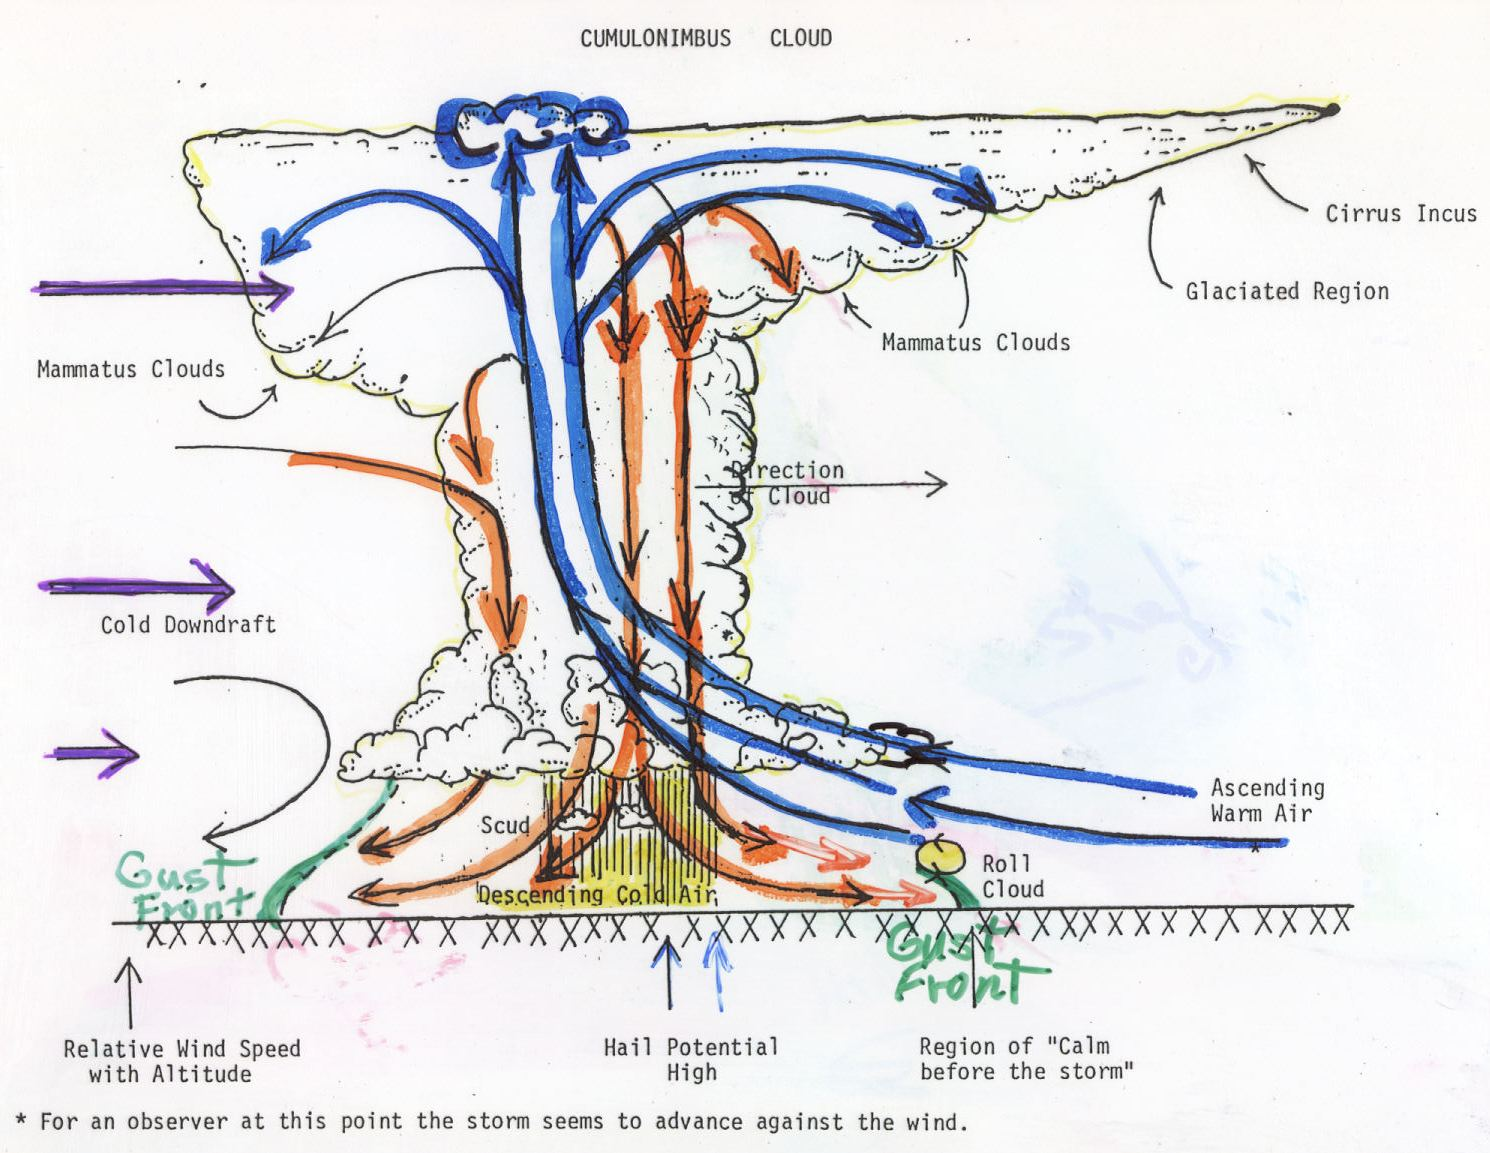
\includegraphics[width=\linewidth]{cloud}
    \caption{}
    \label{fig:cloud}
\end{figure*}
\begin{figure*}[t]
    \centering
    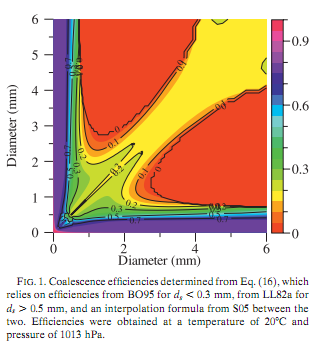
\includegraphics[width=0.75\linewidth]{coalesce_efficiency}
    \caption{}
    \label{fig:coalesce}
\end{figure*}
\begin{figure}[h]
    \centering
    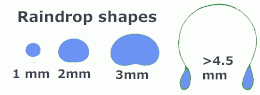
\includegraphics[width=0.75\linewidth]{raindrop_shapes}
    \caption{}
    \label{fig:raindrop}
\end{figure}
\begin{figure*}[t]
    \centering
    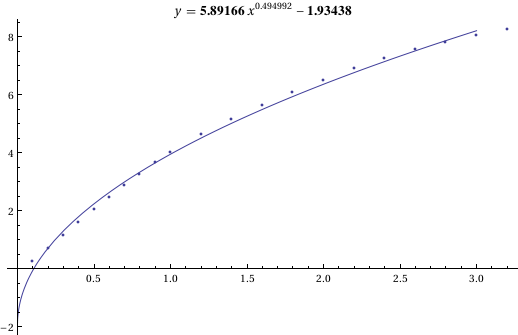
\includegraphics[width=0.75\linewidth]{terminal_velocity}
    \caption{}
    \label{fig:velocity}
\end{figure*}


\section{Model Limitations and Assumptions}

The model proposed here is based on a few key simplifications. First, and
perhaps most importantly, we limit ourselves to a two-dimensional rectangular
domain which significantly taller than it is wide. This shape is a loose
interpretation of the relevant shape of a cloud from the perspective of a single
raindrop, but necessarily ignores factors such as neighboring cloud
interactions and the often significant lateral wind, which ``rolls'' in a cyclic
pattern at the edges of a towering cloud.

A second major assumption is that amount of aerosol in the air remains constant.
This is *known* to be false as airborne particulate counts are shown to be at
their lowest, and visibility at its highest, after a rain event has pulled the
aerosols to the ground. This is important because it affects the likelihood of
new drops forming by reducing the available condensation nuclei. In this
simulation, the rate at which new drops appear is a constant function of the
humidity, and thus implicitly assumes a constant aerosol density and size
distribution.


\section{Erlang}

Erlang is a high level functional language, originally developed by Eriksson in
the 1990's to handle telecommunications workloads. It has since grown to enjoy
wide-spread use in the telecommunications industry as the workhorse runtime in
switches and interchanges. To this end, it has been designed from the ground up
with a strong focus on concurrency, fault-tolerance, and, somewhat unlike its
academic brethren, practicality.

From the perspective of the scientific programmer, working in FORTRAN or C,
Erlang has very different and confusing semantics. In this section, I will try
to address the more obvious quirks and argue my case for choosing Erlang as a
potentially valuable tool in the scientific computing arena.

\subsection{Why not C?}

When we were all introduced to algebra at the beginning of our scientific
careers, we learned that abstract representations of values such as $x$ were
constant. Given two equations, $x = 3$ and $y = x$, we could say with confidence
that $y = 3$ as well. This gave us very powerful tools for reasoning about
complex systems of equations. We could directly substitute variables for their
values, which might again be expressed in terms of variables. This is referred
to as \emph{referential transparency}.

Unfortunately, when we all learned our first programming language, we were told
that \emph{referential transparency} was no longer the way things worked.
Suddenly, expressions like $X = X + 1$ were claimed to make sense and stranger
still, this was considered a great and useful trick when writing programs.
Imperative (read: sequential) languages like C and Java take this abandonment of
mathematics to the extreme. It is virtually impossible to program these
languages without making use of dynamically valued variables. As one might
expect, by relaxing the notion that $x = x$ for any two instances of $x$ in the
same context, referential transparency was lost and the ability to reason about
the correctness of a program disappeared with it. We haven't even begun
discussing the difficulty of reasoning about \emph{concurrent} algorithms
written in this style. The good news is that many very talented people have put
a heroic effort into writing programs in these languages which, almost by magic,
produce mathematically accurate results. The bad news is that, typically, we are
not those people. For you and I, the Programming Scientists, writing non-trivial
programs in C which produce valid results is difficult and extremely time
consuming. Personal experience and informal survey of my own colleagues suggests
that upwards of 90\% of the time spent ``programming'' is actually spent
searching for and correcting the inadvertent effects of changing the value of
variables.

\subsection{Single Assignment Variables}

The irony, of course, is that we are specifically interested in
\emph{mathematical} programming. Fortunately, there has been a minor revival of
the functional programming movement lately. Highly specialized languages such as
Mathematica provide a gentle reintroduction to mathematical programming for
those who have forgotten their algebraic roots\footnote{Pun intended.}. These
languages do suffer from their own problems, however. As demand for large-scale
simulation increases with computing power, the need for parallel algorithms that
can exploit multiple concurrent threads of execution become grows with it.
Equally important is the ability of the programmer to successfully implement
these algorithms.

\subsection{Pattern Matching}

This feature, common to many functional languages, is a way of selecting a
particular implementation of a function based not only on the types of the
arguments passed to it, commonly referred to as ``overloading'', but also the
values of those arguments. In Erlang, this manifests as the widespread use of a
language feature called ``atoms''. Atoms are simply C-like identifiers that
begin with a lowercase letter and have no value other than their name. They are
used extensively to ``tag'' other values and then pass them to a function which
implicitly chooses the correct  definition based on equality testing against the
tag.
For example, a function which acts upon possible events in a simulation,
might receive a tuple consisting of a tag denoting the event type and a value
representing the event itself, such as \texttt{(create, 42)}.

A second important feature of pattern matching is its ability to bind variable
names to values, even deep inside complicated types. For example, a function
which expects to pattern match against a tuple of values might declare it's
arguments to be of type \texttt{(Arg1, Arg2)}. In this case, the match will only
succeed against a single 2-tuple (as opposed to two separate function arguments),
whereupon the first value of the tuple will be bound to the name Arg1 and the
second to Arg2. In practice, this simple concept provides a great deal of
type-safety and sanity checking throughout the code. It is yet another reason
that proponents of functional languages based on pattern matching claim to spend
less time debugging and provide guarantees of correctness. Personally, I find it
to be a very useful technique, which indeed caught many problems right at
function interfaces, decreasing uncertainty about the true origin of bugs.

\section{Implementation}


As stated previously, maintaining scalability with respect to performance was a
key goal of this project. To that end, I chose to model the computational domain
as a monoid based on quadtrees, a tree-like partitioning method based on data
location and density.

\subsection{Domain as a forest of quadtrees}

The computational domain, ``the sky'', is represented by a collection of
quadtree. This is simply a tree in which every node has exactly four children,
representing the four quadrants of a rectangular subdomain. These in turn are
nodes themselves which can be further subdivided as necessary. A strict
definition of quadtrees requires that each subdomain be so divided until it
contains a single data point, \autoref{fig:quadtree}. From an efficiency
perspective, this is not ideal and instead, I use a generalized quadtree wherein
nodes may contain either four children or a collection of between 0 and $N$
points, representing rain drops.

\begin{figure}[h]
    \centering
    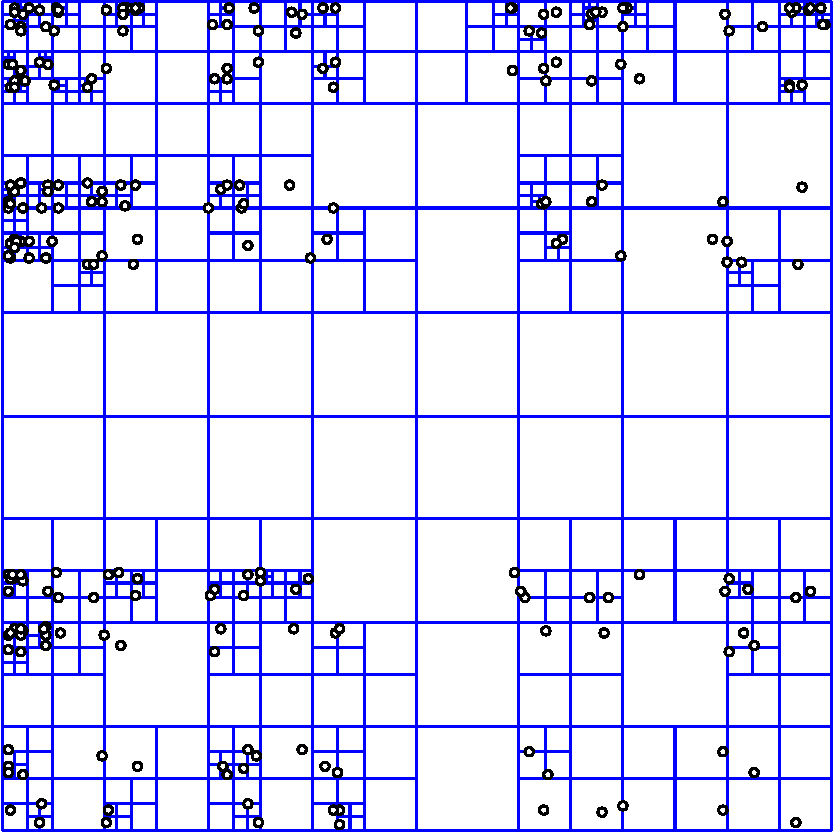
\includegraphics[width=0.75\linewidth]{quadtree}
    \caption{A quadtree showing subdomains restricted to contain at most a
    single data point each.}
    \label{fig:quadtree}
\end{figure}

What's nice about this representation is that it an incremental way of
dynamically repartitioning it falls out from the definition. Since the quadtree
divides every domain into four equally sized subdomains, we can simply combine a
subdomain with its three siblings again when the total number of points among
the four falls below $N$. Similarly, if any subdomain contains more than $N$
points, it can be split into four grandchildren, independent of the neighboring
subdomains. We simply define a function
\begin{verbatim}
split : QT -> (QT, QT, QT, QT)
\end{verbatim}
and its inverse
\begin{verbatim}
merge : (QT, QT, QT, QT) -> QT
\end{verbatim}
such that \texttt{merge(split(x)) = x}. Then apply them as necessary to keep the
number of points in a subdomain below $N$.

Now with a tiny bit of extra work communicating points from bordering regions,
we can independently work inside of all subdomains concurrently. Indeed,
\emph{this} is the original motivation for testing a language like Erlang on
this problem. I believe that the message passing, massively concurrent style of
Erlang programming is a great fit.

Our simulation will run as a collection of stochastic cellular automata. Each
cell containing potentially multiple drops, each of which follows a random walk
in addition to deterministic environment factors such as gravity and wind
interaction.


\subsection{Expert Knowledge and Rules}
\label{sec:rules}

The deterministic aspect of the simulation, as well as many parameters from the
stochastic aspect, come from the admittedly shallow body of literature
surrounding the physics of rain itself. We classify a droplet as ``rain'' when
it attains a size of 0.5mm or greater. \citet{hu1998} provides interpolated
values for the likelihood of drops to coalesce when touching one another,
referred to \emph{coalescence efficiency}.

As the snippet in \autoref{fig:coalesce} shows, very small drops, less than
0.5mm, are more likely to coalesce than any other, but the drop in efficiency
above that line is very sharp. For larger drops, difference in drop diameter is
strongly inversely correlated with coalescence efficiency. These qualities
suggest that large numbers of small droplets should be produced, with very few
large droplets forming.




\subsection{Performance}

Erlang is not known for its high computational throughput. For
example, the language has no native support for arrays, relying instead on
linked lists and hash tables. This presented a serious problem when working with
collections of raindrops in my simulation. I certainly could not afford the poor
lookup times of linked lists and so I represented drop collections as hash
tables, keyed on the location of the drop.

\subsubsection{HiPE}

In an attempt to address Erlang's performance issues, an optimizing compiler
Referred to as Hi-Performance-Erlang (HiPE), was developed \cite{hipe}. This
compiler produces native machine code as opposed to bytecode for the BEAM
virtual machine, which makes compiled programs non-portable. It does provide a
significant boost to performance. Numerically intense code can see speedup in
the range of 5 to 10 times faster than the interpreted BEAM code. In some cases
this can be superior to the speed of implementations in interpreted languages,
such as Python. Unfortunately, Python is not known for speed when running
numerically intensive algorithms.









\clearpage
\nocite{*}
\bibliographystyle{unsrtnat}
\bibliography{Modeling_the_Formation_of_Rain.bib}
\end{document}


